\documentclass{beamer}
\usepackage[english]{babel}
\usepackage{graphicx}

%%%%%%%%%% Start TeXmacs macros
\newenvironment{itemizearrow}{\begin{itemize} \renewcommand{\labelitemi}{$\rightarrow$}\renewcommand{\labelitemii}{$\rightarrow$}\renewcommand{\labelitemiii}{$\rightarrow$}\renewcommand{\labelitemiv}{$\rightarrow$}}{\end{itemize}}
\newenvironment{itemizedot}{\begin{itemize} \renewcommand{\labelitemi}{$\bullet$}\renewcommand{\labelitemii}{$\bullet$}\renewcommand{\labelitemiii}{$\bullet$}\renewcommand{\labelitemiv}{$\bullet$}}{\end{itemize}}
%%%%%%%%%% End TeXmacs macros

\begin{document}

{\screens{\

\

\

\

\

\title{计算视觉与模式识别}

\maketitle

\ }{\begin{frame}
  \frametitle{百闻不如一见}
  
  \resizebox{1\columnwidth}{!}{\includegraphics{img/qingmingshanghetu.png}}
\end{frame}}{\begin{frame}
  \frametitle{耳听为虚,眼见为实?}
  
  \quad\resizebox{0.8\columnwidth}{!}{\includegraphics{img/huananhu.png}}
  
  \qquad https://iask.sina.com.cn/d-b/554b06f3e4b0d8ec5b976531-7.html
\end{frame}}{\begin{frame}
  \frametitle{视觉}
  
  \qquad\resizebox{0.9\columnwidth}{!}{\includegraphics{img/plant_recognition.png}}
\end{frame}}{\begin{frame}
  \frametitle{视觉系统}
  
  \qquad\resizebox{0.9\columnwidth}{!}{\includegraphics{img/phone.png}}
\end{frame}}{\begin{frame}
  \frametitle{视觉系统}
  
  \qquad\resizebox{0.8\columnwidth}{!}{\includegraphics{img/raspberrypi.png}}
  
  \ 
\end{frame}}{\begin{frame}
  \frametitle{开发示例}
  
  {\hspace{3em}}\resizebox{.8\columnwidth}{!}{\includegraphics{img/servo.png}}
  
  \ 
\end{frame}}{\begin{frame}
  \frametitle{硬件}
  
  \qquad\resizebox{0.8\columnwidth}{!}{\includegraphics{img/servo_hardware.png}}
  
  \ 
\end{frame}}{\begin{frame}
  \frametitle{软件}
  
  \qquad\resizebox{0.8\columnwidth}{!}{\includegraphics{img/servo_software.png}}
\end{frame}}{\begin{frame}
  \frametitle{流程图}
  
  {\hspace{4em}}\resizebox{0.6\columnwidth}{!}{\includegraphics{img/servo_flowchart.png}}
\end{frame}}{\begin{frame}
  \frametitle{应用示例------三维重建}
  
  \qquad\resizebox{0.8\columnwidth}{!}{\includegraphics{img/3d_reconstruction.png}}
\end{frame}}{\begin{frame}
  \frametitle{}
  
  \qquad\resizebox{0.9\columnwidth}{!}{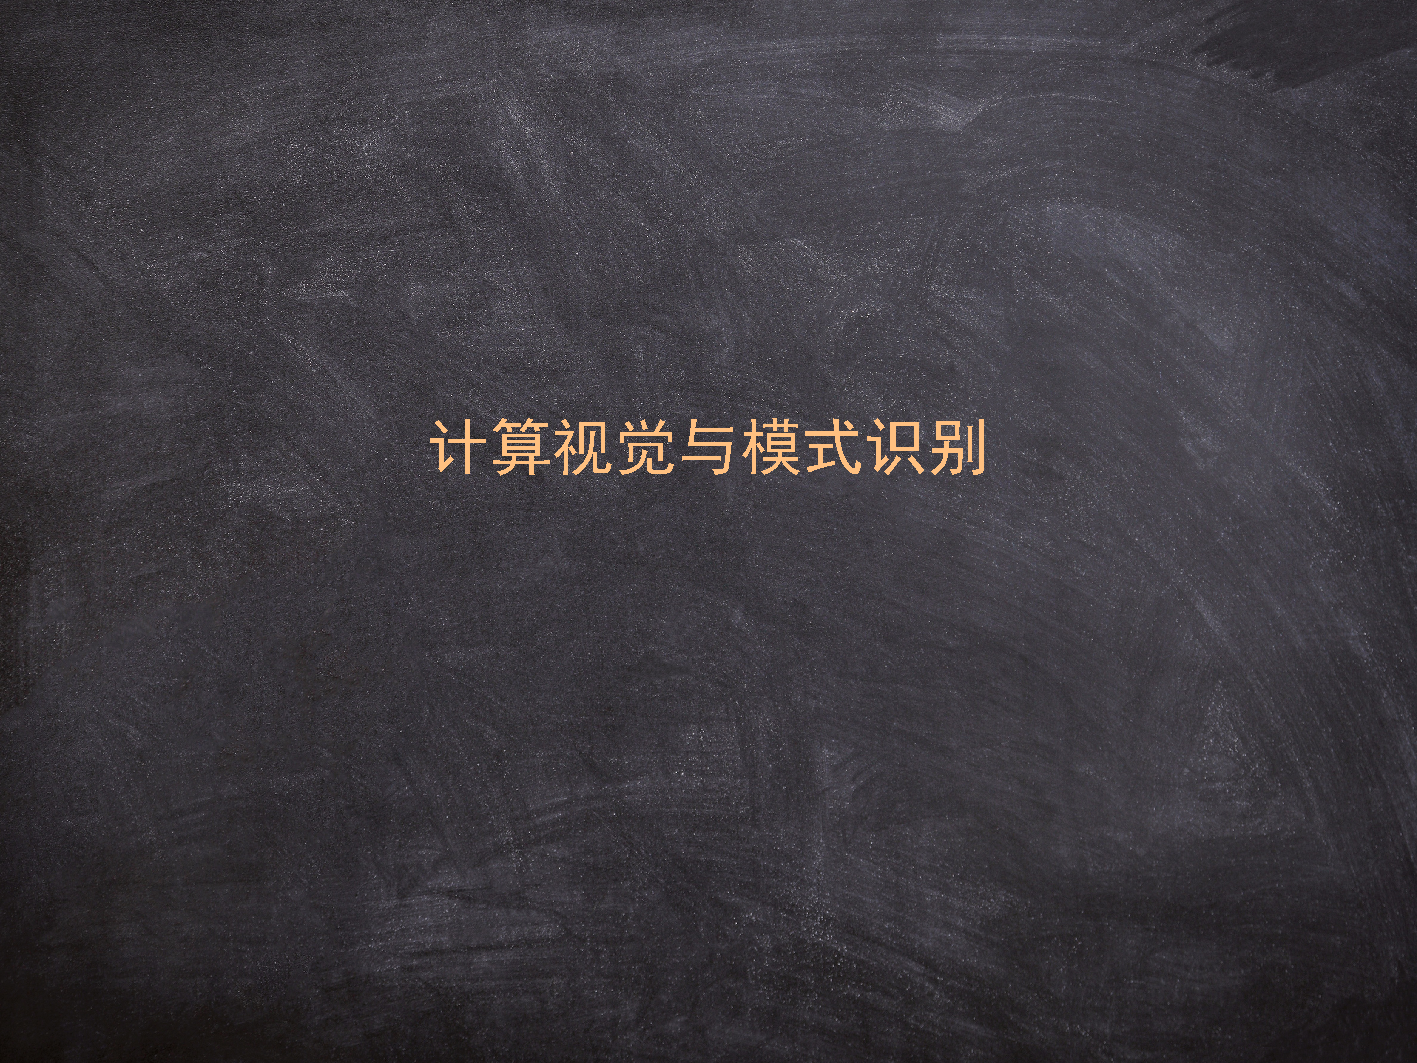
\includegraphics{img/calibration.png}}
\end{frame}}{\begin{frame}
  \frametitle{}
  
  \qquad\resizebox{0.9\columnwidth}{!}{\includegraphics{img/3d_multi_image.png}}
\end{frame}}{\begin{frame}
  \frametitle{}
  
  \qquad\resizebox{0.8\columnwidth}{!}{\includegraphics{img/3d_reconstruction_result.png}}
\end{frame}}{\begin{frame}
  \frametitle{应用示例------姿态估计}
  
  \resizebox{0.9\columnwidth}{!}{\includegraphics{img/pose.png}}
  
  \ 
\end{frame}}{\begin{frame}
  \frametitle{模糊恢复}
  
  \quad\resizebox{0.9\columnwidth}{!}{\includegraphics{img/deblur.png}}
\end{frame}}{\begin{frame}
  \frametitle{运动分析}
  
  \resizebox{1\columnwidth}{!}{\includegraphics{img/motion1.png}}
\end{frame}}{\begin{frame}
  \frametitle{}
  
  {\hspace{4em}}\resizebox{0.8\columnwidth}{!}{\includegraphics{img/motion2.png}}
\end{frame}}{\begin{frame}
  \frametitle{应用示例------人脸识别(训练)}
  
  {\hspace{4em}}\resizebox{0.7\columnwidth}{!}{\includegraphics{img/face_recognition_train.png}}
\end{frame}}{\begin{frame}
  \frametitle{}
  
  {\hspace{4em}}\resizebox{0.7\columnwidth}{!}{\includegraphics{img/eigenface.png}}
\end{frame}}{\begin{frame}
  \frametitle{应用示例------人脸识别(测试)}
  
  {\hspace{4em}}\resizebox{0.7\columnwidth}{!}{\includegraphics{img/face_recognition_test.png}}
\end{frame}}{\begin{frame}
  \frametitle{手写识别}
  
  \qquad\resizebox{0.8\columnwidth}{!}{\includegraphics{img/lenet.png}}
\end{frame}}{\begin{frame}
  \frametitle{应用示例------分割}
  
  {\hspace{3em}}\resizebox{0.6\columnwidth}{!}{\includegraphics{img/segmentation.png}}
\end{frame}}{\begin{frame}
  \frametitle{应用示例------目标检测}
  
  {\hspace{5em}}\resizebox{0.7\columnwidth}{!}{\includegraphics{img/detection.png}}
\end{frame}}{\begin{frame}
  \frametitle{应用示例------目标跟踪}
  
  \qquad\resizebox{0.7\columnwidth}{!}{\includegraphics{img/tracking.png}}
\end{frame}}{\begin{frame}
  \frametitle{马尔计算视觉}
  
  视觉主要功能在于:
  
  {\hspace{4em}}从视网膜成像的二维图像来恢复空间物体的可见三维表面形状'',
  
  即``三维重建''(3D reconstruction)。
  \begin{itemizedot}
    \item 计算理论
    
    挖掘关于成像物理场景的内在属性来完成相应的视觉问题计算
    
    \item 表达和算法
    
    物体的表达形式为该物体的三维几何形状。
    
    \item 算法实现
    
    大脑的神经计算和计算机的数值计算没有本质区别
  \end{itemizedot}
  
  
  \ 
\end{frame}}{\begin{frame}
  \frametitle{表达和算法}
  
  {\hspace{3em}}从图像到三维表达,要经过三个计算层次:
  
  
  \begin{enumerate}
    \item 从图像得到一些基元(primal sketch),
    
    \item
    通过立体视觉(stereopsis)等模块将基元提升到2.5维表达,
    
    \item 提升到三维表达。
  \end{enumerate}
\end{frame}}{\begin{frame}
  \frametitle{相关学科}
  
  \quad\resizebox{0.8\columnwidth}{!}{\includegraphics{img/relation.png}}
\end{frame}}{\begin{frame}
  \frametitle{课程内容}
  \begin{itemizedot}
    \item 摄像机模型
    
    \item 图像特征提取
    
    \item 图像配准与拼接
    
    \item 立体视觉
    
    \item 模式识别基础
    
    \item 图像目标识别
    
    \item 运动分析
  \end{itemizedot}
\end{frame}}{\begin{frame}
  \frametitle{课程}
  \begin{itemizedot}
    \item https://www.coursera.org/learn/digital
    
    Fundamentals of Digital Image and Video Processing(coursera)
    
    \item https://www.coursera.org/learn/image-processing
    
    Image and Video Processing: From Mars to Hollywood with a Stop at
    
    the Hospital(coursera)
    
    \item https://www.coursera.org/learn/computer-vision-basics
    
    Computer Vision Basics University at Buffalo
  \end{itemizedot}
\end{frame}}{\begin{frame}
  \frametitle{\ }
  \begin{itemizedot}
    \item https://github.com/kmario23/deep-learning-drizzle
    \begin{itemizearrow}
      \item https://vision.in.tum.de/teaching/ws2016/vmcv2016
      
      \item https://web.eecs.umich.edu/\~{}justincj/teaching/eecs498/WI2022/
      
      \item
      https://www.crcv.ucf.edu/courses/cap5415-fall-2020/material-cap5415-fall-2020/
    \end{itemizearrow}
  \end{itemizedot}
\end{frame}}{\begin{frame}
  \frametitle{参考资料}
  \begin{itemizedot}
    \item 计算机视觉------一种现代方法
    
    \item Python计算机视觉编程
    
    \item 数字图像处理(冈萨雷斯)
    
    \item 计算机视觉:算法与应用
    
    \item Pattern Recognition and Machine Learning
  \end{itemizedot}
\end{frame}}{\begin{frame}
  \frametitle{软件/程序}
  
  
  \begin{itemizedot}
    \item Python
    
    \item Matlab/Octave
    
    \item Julia
    
    \item R
    
    \item C++
    
    \item Java
  \end{itemizedot}
\end{frame}}{\begin{frame}
  \frametitle{资源}
  
  
  \begin{itemizedot}
    \item https://www.kaggle.com/ 数据科学竞赛平台、社区
    
    \item https://learnxinyminutes.com \textbackslash
    各种程序设计语言快速入门
    
    \item https://mirrors.tuna.tsinghua.edu.cn/\quad清华镜像
    
    \item https://mirrors.ustc.edu.cn/\qquad中科大镜像
  \end{itemizedot}
\end{frame}}{\begin{frame}
  \frametitle{软件工具}
  \begin{itemizedot}
    \item http://dlib.net/\qquad machine learning C++ toolkit
    
    \item https://opencv.org/\quad computer vision toolkit
    
    \item https://keras.io/{\hspace{3em}}neural network toolkit
    
    \item https://tensorflow.google.cn/\quad machine learning toolkit
    
    \item https://scikit-image.org/\qquad image processing in python
    
    \item https://pytorch.org/\qquad machine learning toolkit
    
    \item https://www.cimg.eu/\quad c++ template image processing library
  \end{itemizedot}
\end{frame}}{\begin{frame}
  \frametitle{图像处理工具}
  
  
  \begin{itemizedot}
    \item GIMP(GNU Image Manipulation Program):
    
    http://www.gimp.org
    
    \item ImageMagick:
    
    http://www.imagemagick.org
    
    \item ImageJ:
    
    https://imagej.nih.gov/ij/
    
    \item VLFEET:
    
    http://www.vlfeat.org
    
    \ 
  \end{itemizedot}
  
\end{frame}}}

\end{document}
